\documentclass[a4paper]{article}
\usepackage[utf8]{inputenc}
\usepackage{geometry}
\geometry{legalpaper, margin=1in}
\usepackage[T1]{fontenc}
\usepackage{algorithm}
\usepackage[noend]{algpseudocode}
\newcommand\tab[1][1cm]{\hspace*{#1}}
\usepackage{graphicx}

\title{SDD : TP 1}
\author{Mathieu Boutin - Jérémy Morceaux}
\begin{document}
\maketitle
\section{Présentation générale}
- Ce TP à pour but de créer une matrice représentant des coûts de production de différentes usines à différentes périodes depuis un fichier. Il faut ensuite récupérer les K usines ayant le plus faible coût de production. Finalement, il faut toutes les occurences d'une usines u dans cette liste et les supprimer.
\\
\\
- schéma  à terminer.
\\
\\
- Les fichiers sources se trouvent dans le dossier \textbf{src}.Les fonctions relatives au matrices sont dans le fichier \textbf{ZZ\_matrix.c} et les fonctions relatives aux listes chainées sont dans le fichier \textbf{ZZ\_linked\_list.c}. Les entêtes sont dans le dossier \textbf{include}.

\section{Détail de chaque fonction}
\subsection{findElt}
\begin{algorithm}
Principe : FindElt
\\
\\
\tab On initialise un pointeur courant qui va parcourir la liste. 
\\
\tab Tant qu'il n'est pas arrivé à la fin et que l'élément est inférieur à v 

\tab \tab On parcout la liste chainée.
\\
\tab On retourne l'adresse du pointeur courant 

FIN
\end{algorithm}
\underline{Lexique :}
\begin{itemize}
\item Paramètre(s) de la fonction  
\begin{itemize}
\item pHead est la tête fictive de la liste chainée
\item v est la valeur que l'on cherche dans cette liste.
\end{itemize}
\item Variable(s) locale(s)
\begin{itemize}
\item curr est le pointeur courant qui parcourt la liste.
\end{itemize}
\end{itemize}
\underline{Programme commenté :}
\begin{center}
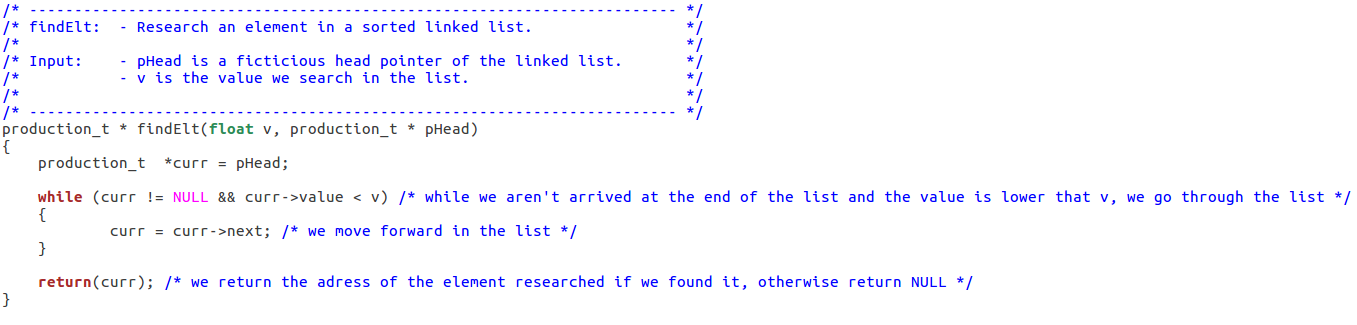
\includegraphics[scale=0.39]{findElt.png}
Source code : findElt()
\end{center}

\subsection{linkBlock}
\begin{algorithm}
Principe : linkBlock
\\
\\
\tab On fait pointer notre nouveau bloc vers suivant
\\
\tab On fait pointer le bloc précédent vers notre nouveau bloc.

FIN
\end{algorithm}
\newpage
\underline{Lexique :}
\begin{itemize}
\item Paramètre(s) de la fonction  
\begin{itemize}
\item prev est le pointeur qui pointe vers l'élément précédent.
\item element est le pointeur vers notre nouveau bloc.
\item next est le pointeur vers le bloc suivant.
\end{itemize}
\end{itemize}
\underline{Programme commenté :}

\begin{center}
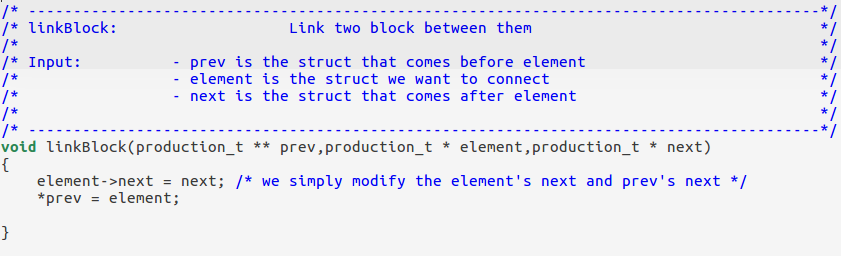
\includegraphics[scale=0.39]{linkBlock.png}

Source code : linkBlock()
\end{center}

\subsection{insertKSorted}
\begin{algorithm}
Principe : insertKSorted
\\
\\
\tab On initialise un pointeur courant et un pointeur qui pointera vers l'élément précédent; 

\tab Si la liste chainée est non vide 

\tab \tab On initialise un compteur à zéro

\tab \tab Tant qu'on est pas à la fin de la liste

\tab \tab \tab On cherche le bloc où l'on doit insérer notre nouveau bloc. A chaque bloc visité, on 
\tab \tab \tab incrémente le compteur 

\tab \tab Si le compteur est inférieur ou égale à K 

\tab \tab \tab Si l'adresse du bloc où l'on doit ajouter le nouveau bloc est nulle 

\tab \tab \tab \tab On ajoute notre bloc à la liste chainée [ c'est le dernier élément ]

\tab \tab \tab Sinon  

\tab \tab \tab \tab On ajoute notre bloc à la liste chainée et on libère le reste 

\tab \tab Sinon [ La valeur du bloc est trop haute ]

\tab \tab \tab On libère le bloc

\tab Sinon [ La liste est vide ]

\tab \tab On ajoute le bloc à la liste chainée. 

FIN
\end{algorithm}
\underline{Lexique :}
\begin{itemize}
\item Paramètre(s) de la fonction  
\begin{itemize}
\item pHead est la tête fictive de la liste chainée
\item address est l’adresse du bloc où l'on doit ajouter le nouveau bloc
\item element est un pointeur le nouveau bloc
\item K est le nombre de plus petit coût de production que l'on veut garder. 
\end{itemize}
\item Variable(s) locale(s)
\begin{itemize}
\item prev est le pointeur qui pointe vers l'élément précédent.
\item curr est le pointeur courant qui parcourt la liste.
\item j est un compteur qui permet de ne pas dépasser la valeur K.
\item tmp est un pointeur temporaire pour libérer la fin de la liste chainée.
\end{itemize}
\end{itemize}

\underline{Programme commenté :}
\begin{center}
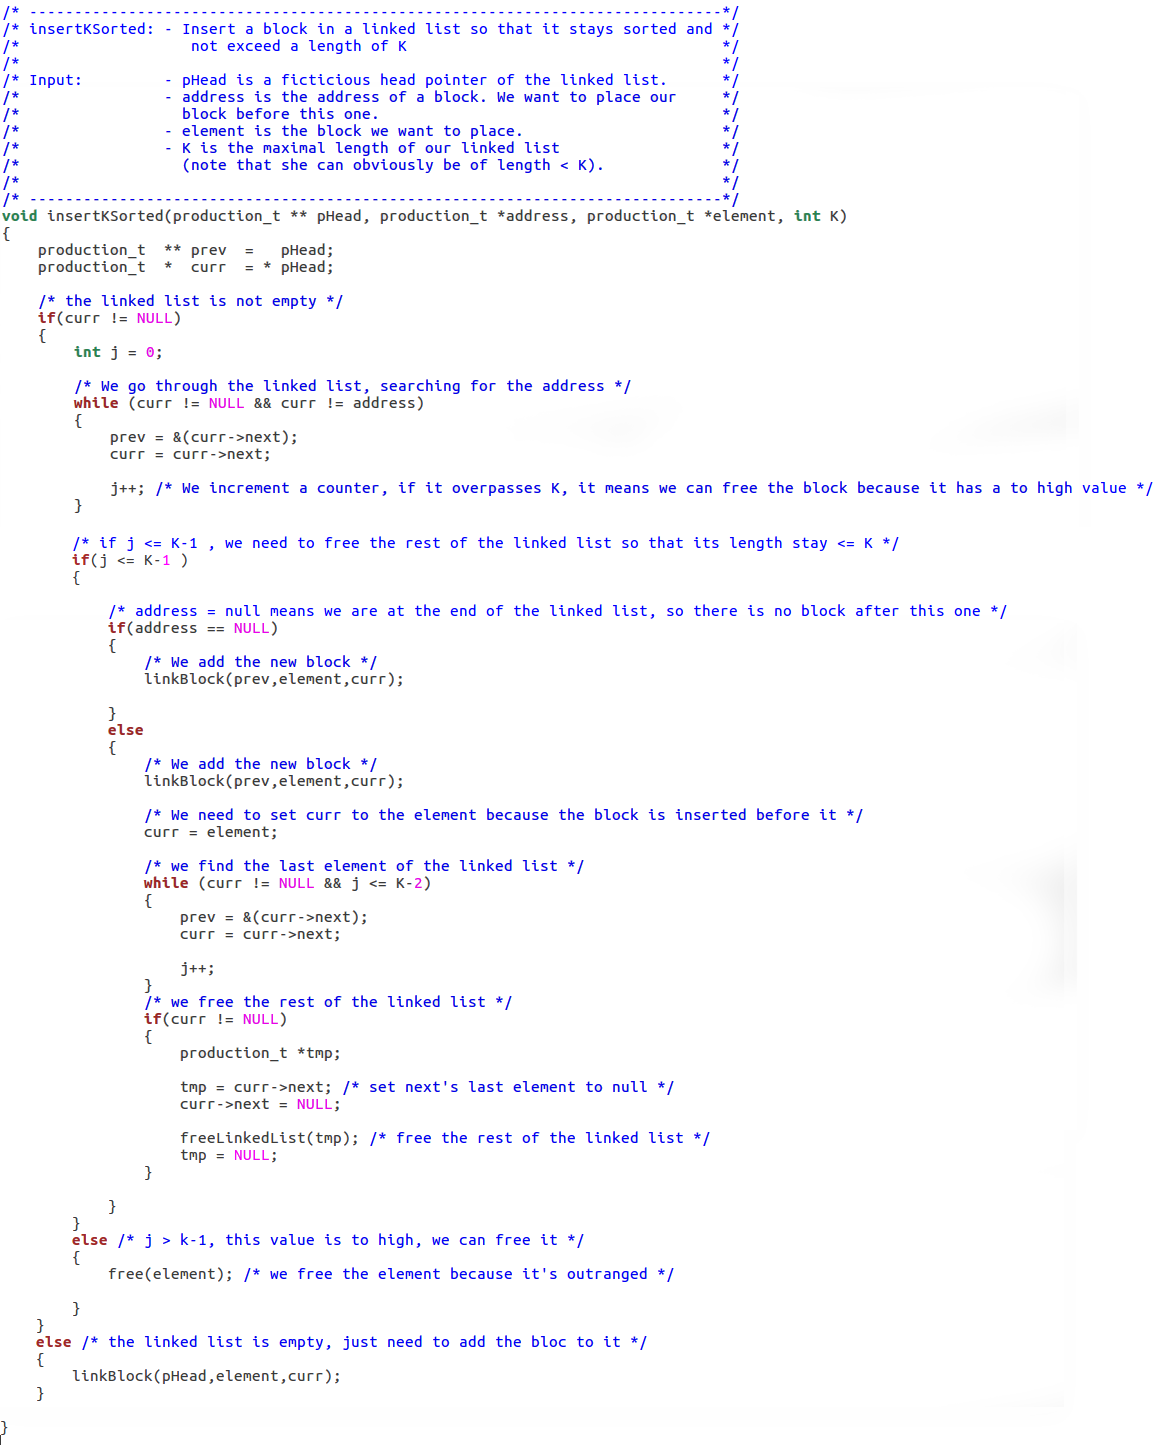
\includegraphics[scale=0.39]{insertKSorted.png}

Source code : insertKSorted()
\end{center}
\subsection{removeFactory}
\begin{algorithm}
Principe : removeFactory
\\
\\
\tab On initialise un pointeur courant, un pointeur précédent et un pointeur temporaire. 

\tab Tant qu'on est pas arrivé à la fin de la liste.

\tab \tab Si l'entreprise courante est celle recherchée alors : 

\tab \tab \tab On supprime cet élément de la liste.

\tab \tab Sinon

\tab \tab \tab On avance dans la liste.

FIN
\end{algorithm}

\underline{Lexique :}
\begin{itemize}
\item Paramètre(s) de la fonction  
\begin{itemize}
\item pHead est la tête fictive de la liste chainée
\item factory est l'indice de l'usine que l'on supprimé de la liste chainée.
\end{itemize}
\item Variable(s) locale(s)
\begin{itemize}
\item prev est le pointeur qui pointe vers l'élément précédant le pointeur curr.
\item curr est le pointeur courant qui parcourt la liste.
\item tmp est un pointeur qui permet de libérer un bloc proprement.
\end{itemize}
\end{itemize}

\underline{Programme commenté :}
\begin{center}
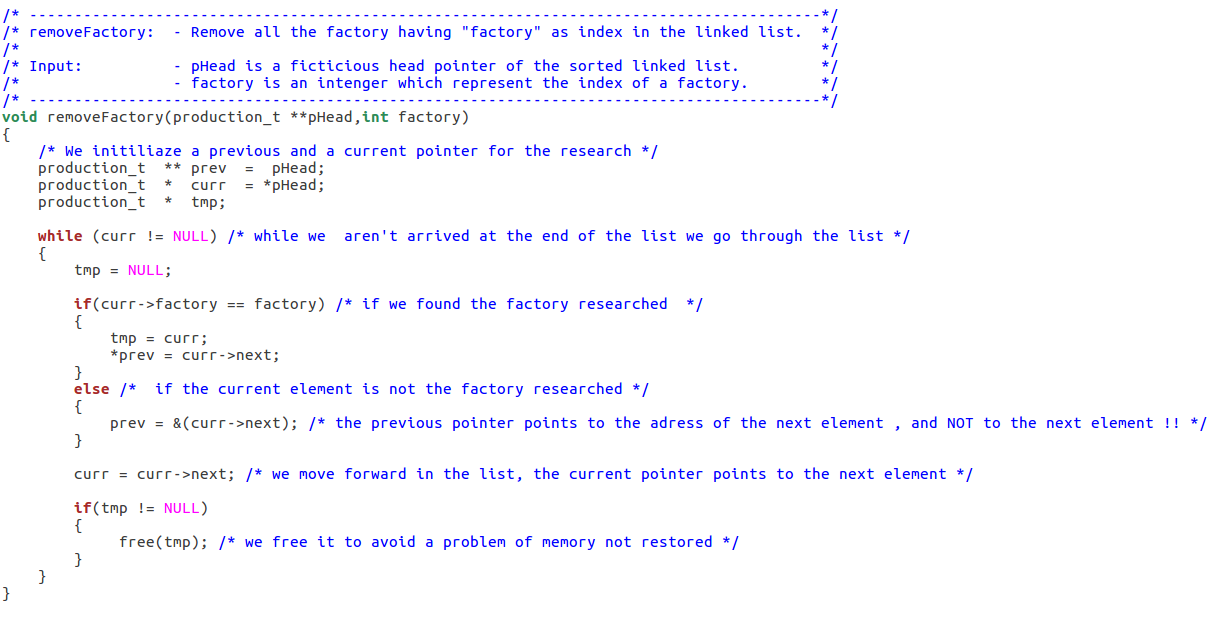
\includegraphics[scale=0.39]{removeFactory.png}

Source code : removeFactory()
\end{center}

\subsection{writeLinkedListToFile}
\begin{algorithm}
Principe : writeLinkedListToFile
\\
\\
\tab On initialise un pointeur courant

\tab Tant qu'on est pas arrivé à la fin de la liste 

\tab \tab On affiche un message avec des données de l'élément courant

\tab \tab Le pointeur courant avance dans la liste 

FIN
\end{algorithm}

\underline{Lexique :}
\begin{itemize}
\item Paramètre(s) de la fonction  
\begin{itemize}
\item file est le fichier dans lequel on veut afficher la liste chainée. (stdout, stderr, ou un fichier texte).
\item pHead est la tête fictive de la liste chainée.
\end{itemize}
\item Variable(s) locale(s)
\begin{itemize}
\item curr est le pointeur courant qui parcourt la liste.
\end{itemize}
\end{itemize}

\underline{Programme commenté :}
\begin{center}
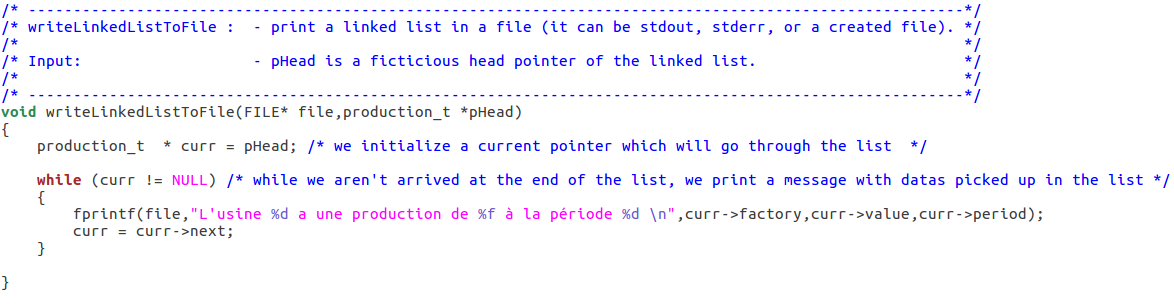
\includegraphics[scale=0.39]{writeLinkedListToFile.png}

Source code : writeLinkedListToFile()
\end{center}

\subsection{insertProductionBlock}
\begin{algorithm}
Principe : insertProductionBlock
\\
\\
\tab On récupère l'adresse à laquelle on doit insérer le nouvel élément afin de garder la liste triée.

\tab On crée un nouveau bloc.

\tab Si on est capable d'allouer le bloc alors

\tab \tab On affecte les nouvelles valeurs à ce bloc.

\tab \tab On l'insert dans la liste chaînée triée.

\tab Sinon 

\tab \tab On affiche un message d'erreur

FIN
\end{algorithm}

\underline{Lexique :}
\begin{itemize}
\item Paramètre(s) de la fonction  
\begin{itemize}
\item pHead est la tête fictive de la liste chainée.
\item value est le coût de production de l'usine.
\item factory est l'indice de l'usine.
\item period est la période de production de l'usine.
\item K est le nombre de plus petit coût de production que l'on veut garder.
\end{itemize}
\item Variable(s) locale(s)
\begin{itemize}
\item insertAdress pointe vers le bloc où on doit insérer le nouveau bloc.
\item newElement pointe vers le nouveau bloc.
\end{itemize}
\end{itemize}

\underline{Programme commenté :}
\begin{center}
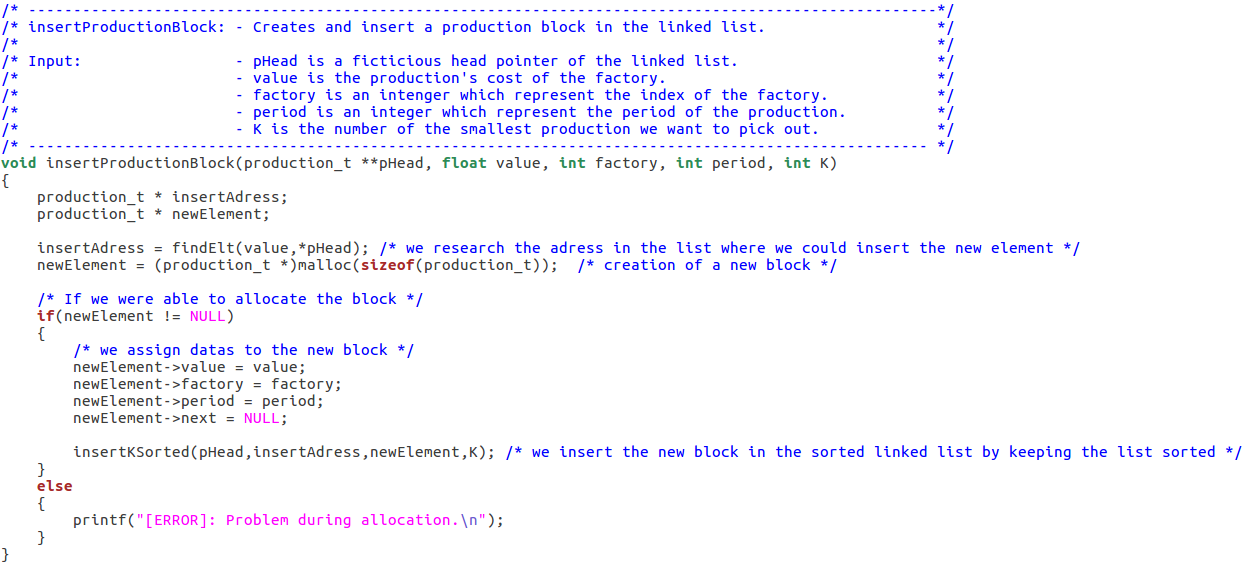
\includegraphics[scale=0.39]{insertProductionBlock.png}

Source code : insertProductionBlock()
\end{center}

\subsection{freeLinkedList}
\begin{algorithm}
Principe : freeLinkedList
\\
\\
\tab Tant qu'on est pas arrivé au bout de la liste faire

\tab \tab On libère proprement le bloc courant.

\tab \tab On passe à l'élément suivant.

FIN
\end{algorithm}

\underline{Lexique :}
\begin{itemize}
\item Paramètre(s) de la fonction  
\begin{itemize}
\item pHead est la tête fictive de la liste chainée.
\end{itemize}
\item Variable(s) locale(s)
\begin{itemize}
\item curr est le pointeur courant qui parcourt la liste.
\item tmp est un pointeur qui permet de libérer un bloc proprement.
\end{itemize}
\end{itemize}

\underline{Programme commenté :}
\begin{center}
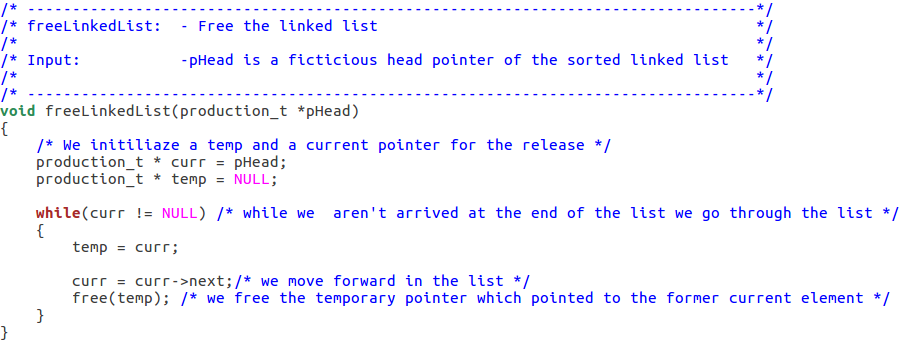
\includegraphics[scale=0.39]{freeLinkedList.png}

Source code : freeLinkedList()
\end{center}

\subsection{loadMatrixFromFile}
\begin{algorithm}
Principe : loadMatrixFromFile
\\
\\
\tab On crée un flux vers notre fichier contenant notre matrice et une matrice pour stocker ses
\tab valeurs, sa ligne, et sa colonne. 
\\
\\
\tab Si le fichier s'est ouvert correctement alors 

\tab \tab On lit les dimensions de la matrice situées sur la première ligne du fichier

\tab \tab On alloue dynamiquement une matrice.

\tab \tab Si on a un problème d'allocation à un certain moment 

\tab \tab \tab on libère proprement la matrice et on rapporte une erreur à la fonction appelante.

\tab \tab Sinon 

\tab \tab \tab On lit l'élément $m_{i,j}$ depuis le fichier et on l'insère dans la matrice 

\tab \tab  On ferme le fichier 

\tab Sinon  

\tab \tab On rapporte une erreur à la fonction appelante.

FIN
\end{algorithm}

\underline{Lexique :}
\begin{itemize}
\item Paramètre(s) de la fonction  
\begin{itemize}
\item fileName est le nom du fichier qui contient la matrice.
\item errorCode est un pointeur sur un entier qui indique si la fonction s'est bien passée.
\end{itemize}
\item Variable(s) locale(s)
\begin{itemize}
\item matrix est une structure contenant les valeurs de la matrice et sa taille.
\item issue = 1, signifie qu'on doit s'arrêter d'allouer la matrice.
\item file est le flux que l'on ouvre avec le nom du fichier contenant la matrice
\item i et j permettent de parcourir la matrice.
\end{itemize}
\end{itemize}

\underline{Programme commenté :}
\begin{center}
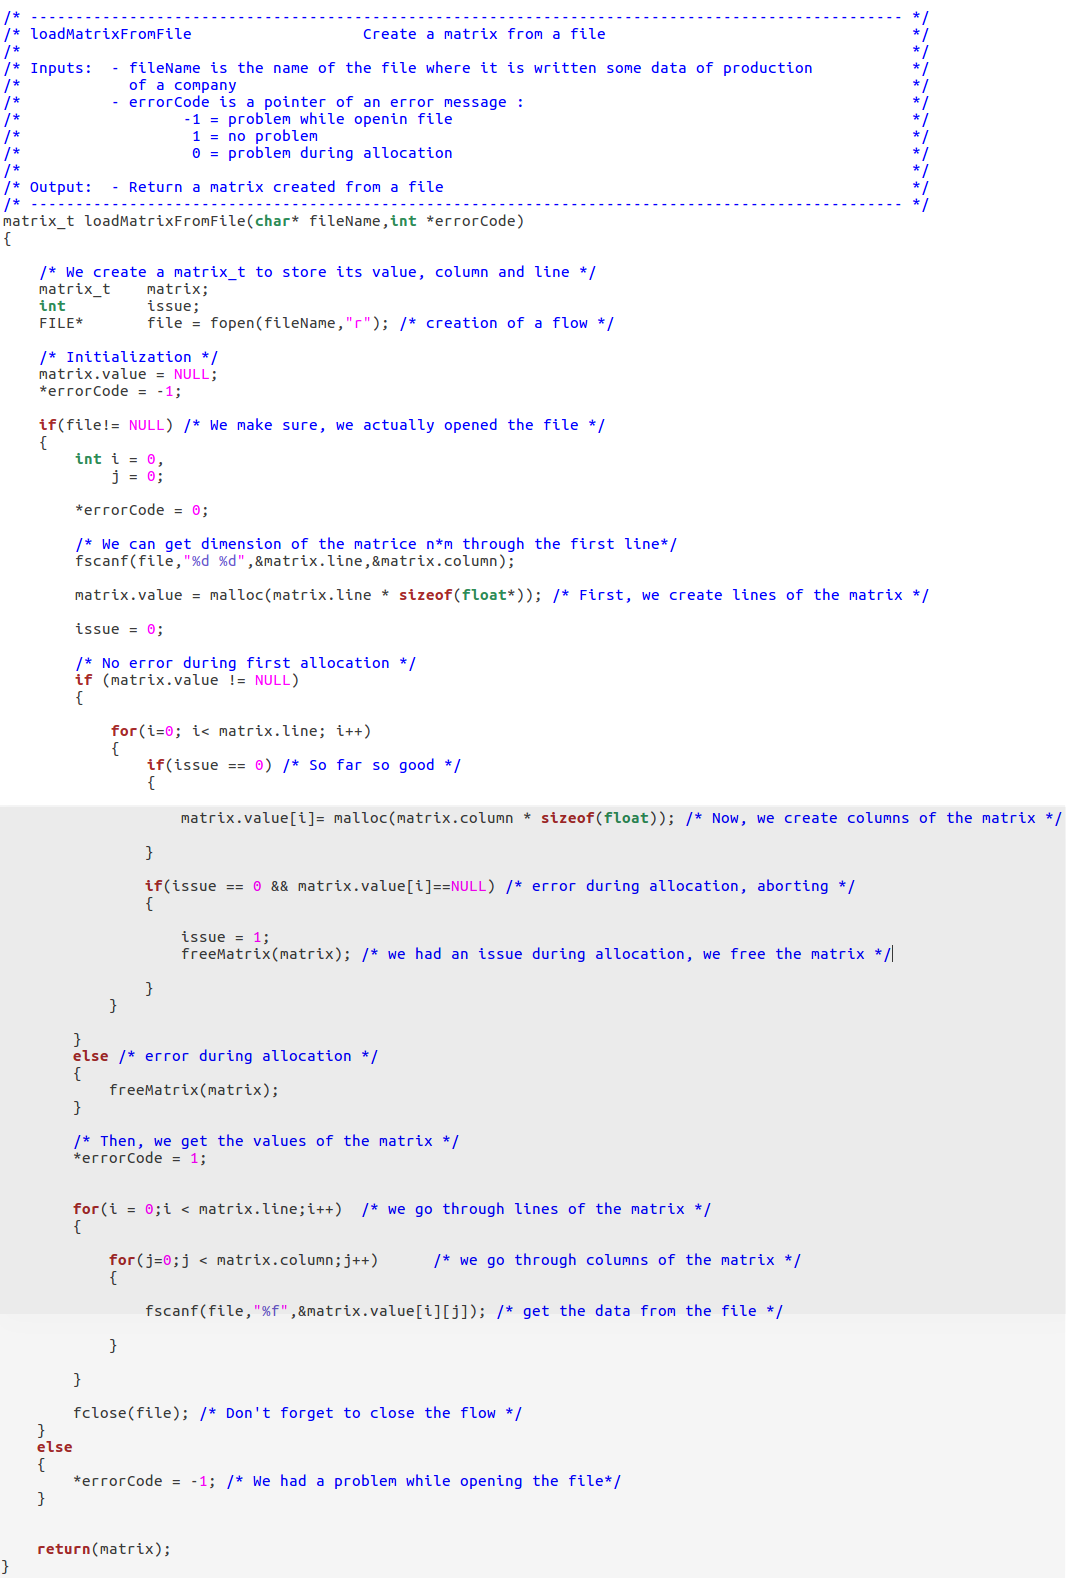
\includegraphics[scale=0.39]{loadMatrixFromFile.png}

Source code : loadMatrixFromFile()
\end{center}

\subsection{freeMatrix}
\begin{algorithm}
Principe : freeMatrix
\\
\\
\tab Si la matrice est non nulle alors : 

\tab \tab On parcourt les lignes de la matrice : 

\tab \tab \tab Si la valeur du bloc de la ligne i est non nulle alors: 

\tab \tab \tab \tab On libère ce bloc

\tab \tab On libère la matrice; 

FIN
\end{algorithm}

\underline{Lexique :}
\begin{itemize}
\item Paramètre(s) de la fonction  
\begin{itemize}
\item matrix est la structure de la matrice que l'on veut afficher
\end{itemize}
\item Variable(s) locale(s)
\begin{itemize}
\item i est l'entier qui permet de supprimer chaque ligne de la matrice.
\end{itemize}
\end{itemize}

\underline{Programme commenté :}
\begin{center}
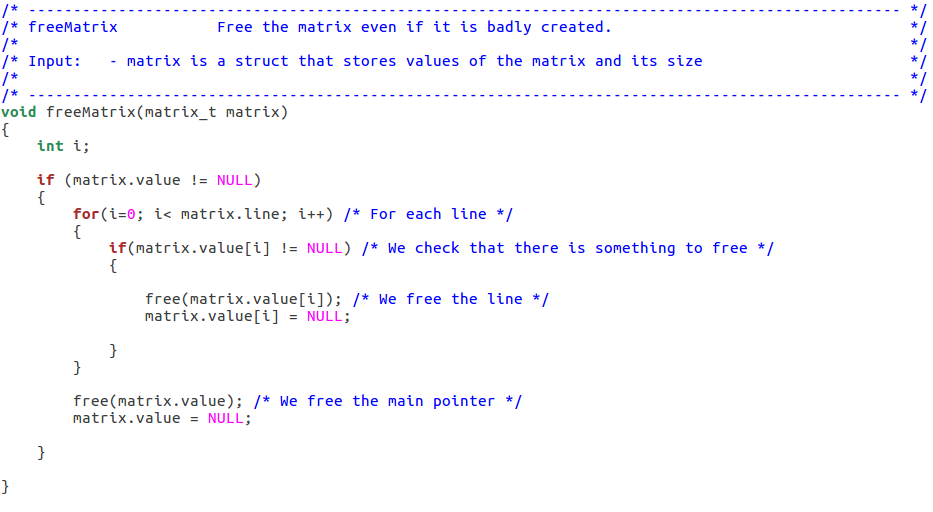
\includegraphics[scale=0.39]{freeMatrix.png}

Source code : freeMatrix()
\end{center}

\subsection{printMatrix}
\begin{algorithm}
Principe : printMatrix
\\
\\
\tab On parcourt les lignes de la matrice

\tab \tab On parcourt les colonnes de la matrice 

\tab \tab \tab On affiche l'élément de la i-ème ligne et de la j-ème colonne 

FIN
\end{algorithm}

\underline{Lexique :}
\begin{itemize}
\item Paramètre(s) de la fonction  
\begin{itemize}
\item matrix est la structure de la matrice que l'on veut afficher.
\end{itemize}
\item Variable(s) locale(s)
\begin{itemize}
\item i et j permettent d'afficher l'élément de la i-ème ligne et de la j-ème colonne.
\end{itemize}
\end{itemize}

\underline{Programme commenté :}
\begin{center}
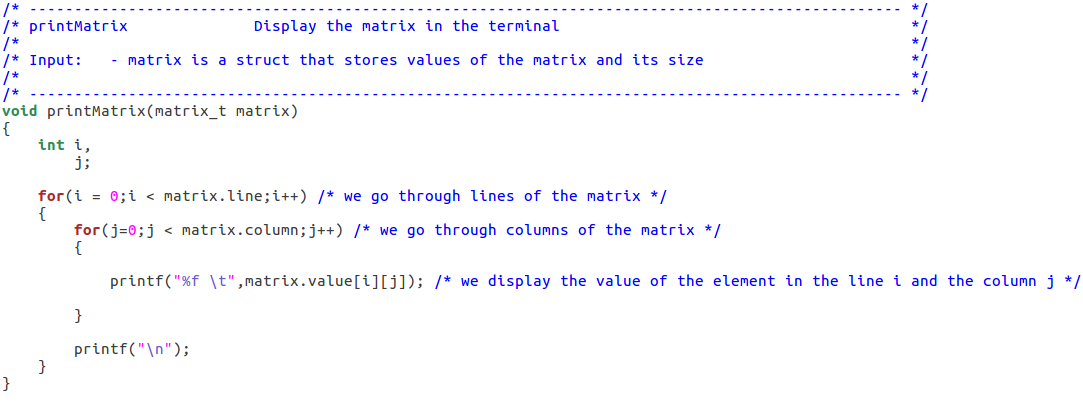
\includegraphics[scale=0.39]{printMatrix.png}

Source code : printMatrix()
\end{center}
\newpage
\subsection{main}
\begin{algorithm}
Principe : main
\\
\\
\tab Si le nombre d'argument est égale à 4 

\tab \tab On crée une matrice à partir du nom de fichier donné en argument 

\tab \tab Si la création s'est bien passée 

\tab \tab \tab On affiche la matrice 

\tab \tab \tab Si K est supérieur à 0 

\tab \tab \tab \tab Si la matrice est non-nulle 

\tab \tab \tab \tab \tab On crée la liste chainée sur toutes les valeurs de la matrice avec 
\tab \tab \tab \tab \tab insertProductionBlock() 

\tab \tab \tab \tab \tab On libère la matrice 

\tab \tab \tab \tab \tab On affiche la liste chainée 

\tab \tab \tab \tab \tab Si l'indice de l'indice a supprimé est valide 

\tab \tab \tab \tab \tab \tab On supprime toutes les occurrences de cette usine dans la liste chainée 

\tab \tab \tab \tab \tab On réaffiche la liste chainée 

\tab \tab \tab \tab \tab On sauvegarde la liste chainée dans un fichier 

\tab \tab \tab \tab \tab On libère la liste chainée 

\tab \tab \tab \tab Sinon 

\tab \tab \tab \tab \tab On prévient l'utilisateur [ Matrice-nulle ! ] 

\tab \tab \tab Sinon 

\tab \tab \tab \tab On prévient l'utilisateur [ K = 0  !! ] 

\tab \tab Sinon  

\tab \tab \tab On prévient l'utilisateur [ Problème d'ouverture de fichier !! ] 

\tab Sinon 

\tab On prévient l'utilisateur [ Pas assez/trop peu d'arguments !! ] 

FIN
\end{algorithm}

\underline{Lexique :}
\begin{itemize}
\item Paramètre(s) de la fonction  
\begin{itemize}
\item argc est le nombre d'arguments du programme.
\item argv est la liste des arguments du programme.
\end{itemize}
\item Variable(s) locale(s)
\begin{itemize}
\item matrixA est la structure de la matrice.
\item codeError enregistre l'état de sortie d'une fonction.
\item i et j permettent de parcourir la matrice.
\item K est le nombre de plus petit coût de production que l'on veut garder.
\item factoryIndex est l'indice de l'usine a supprimée dans la liste chainée.
\item file est le flux pour enregistrer la liste chainée.
\end{itemize}
\end{itemize}

\underline{Programme commenté :}
\begin{center}
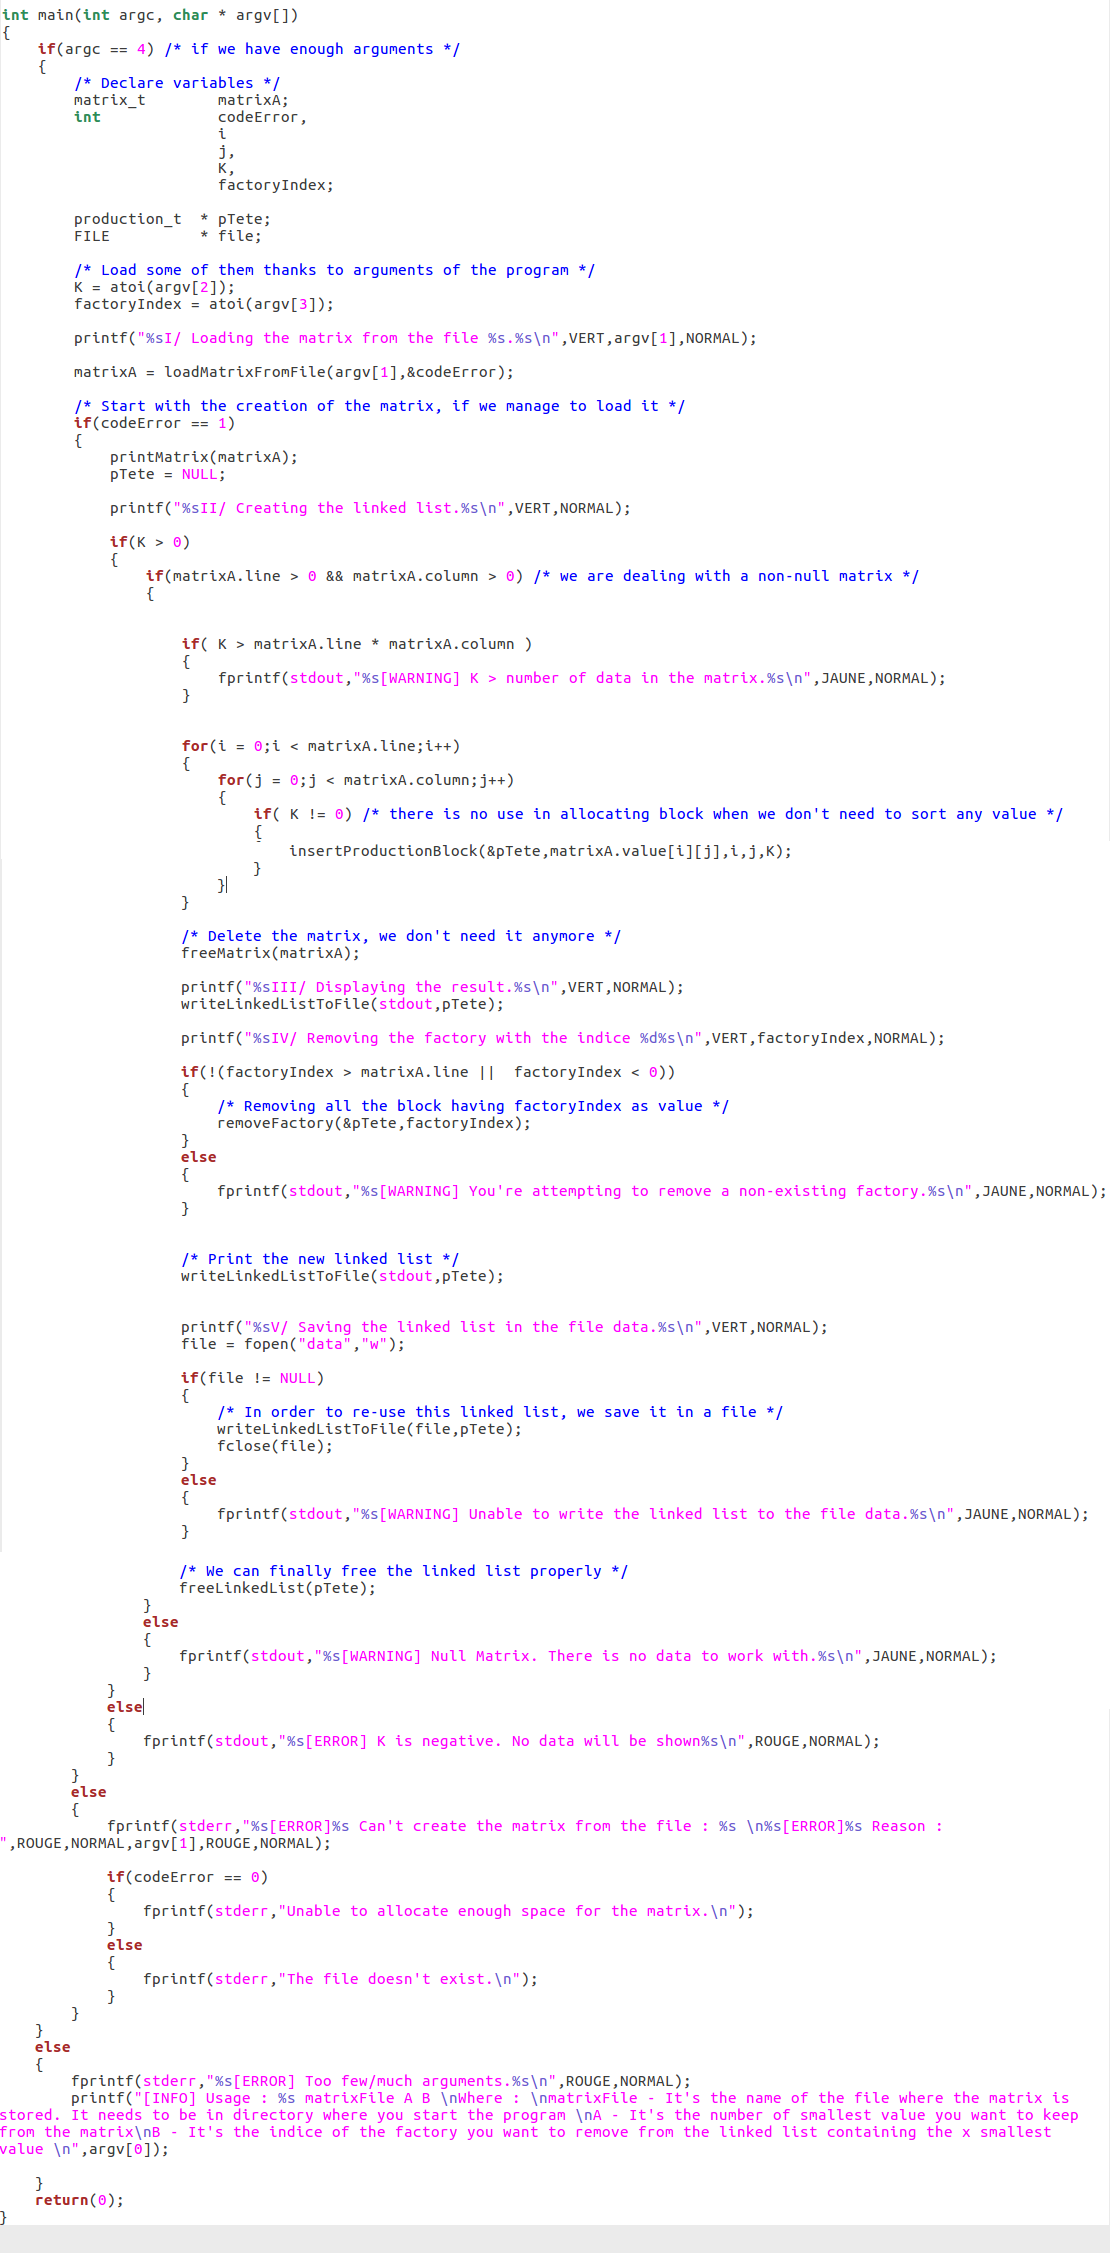
\includegraphics[scale=0.39]{main.png}

Source code : main()
\end{center}
\section{Compte rendu d'exécution}

\underline{Makefile :}
\begin{center}
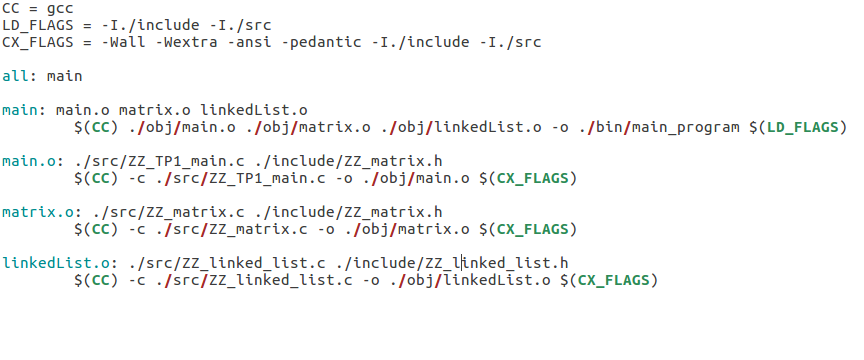
\includegraphics[scale=0.39]{Makefile.png}

figure : Makefile
\end{center}

\underline{Jeux de test complets:}
\begin{center}
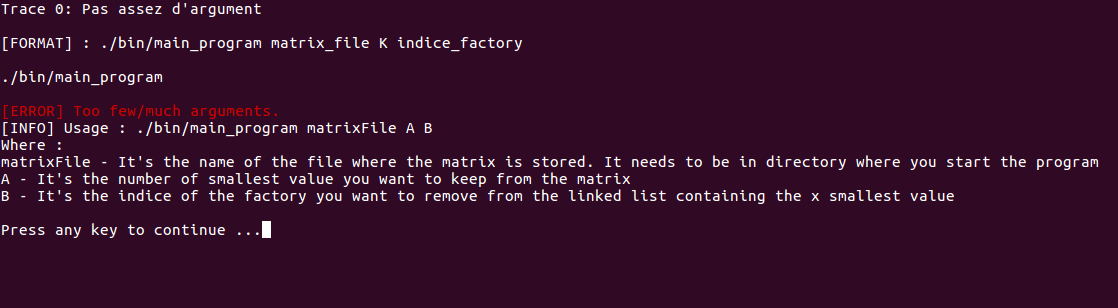
\includegraphics[scale=0.4]{trace_1.png}

figure : Trace 1
\end{center}

\begin{center}
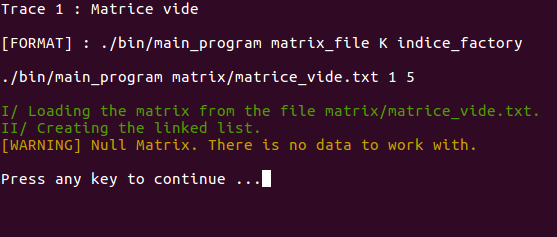
\includegraphics[scale=0.4]{trace_2.png}

figure : Trace 2
\end{center}

\begin{center}
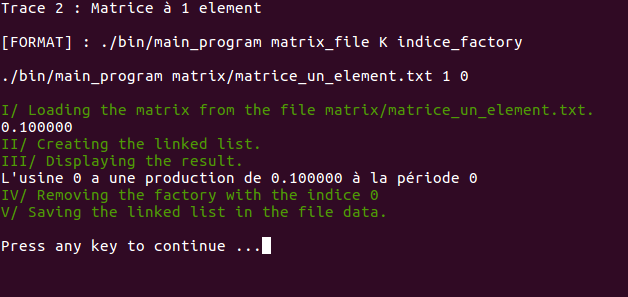
\includegraphics[scale=0.4]{trace_3.png}

figure : Trace 3
\end{center}

\begin{center}
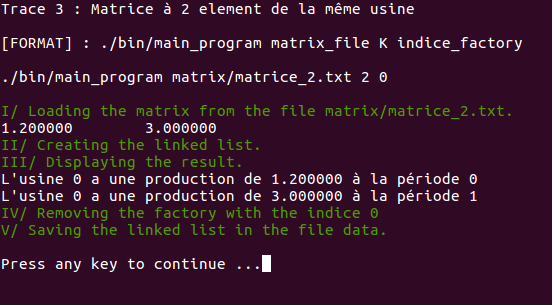
\includegraphics[scale=0.4]{trace_4.png}

figure : Trace 4
\end{center}
\begin{center}
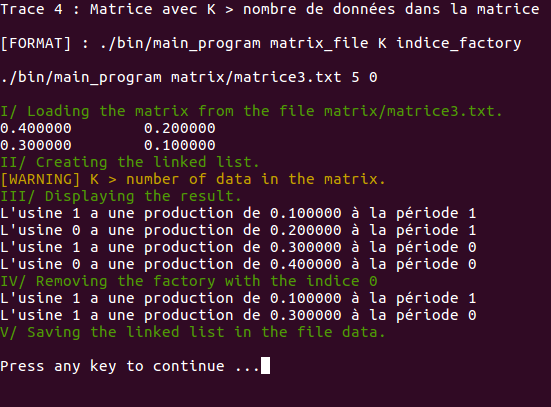
\includegraphics[scale=0.4]{trace_5.png}

figure : Trace 5
\end{center}

\begin{center}
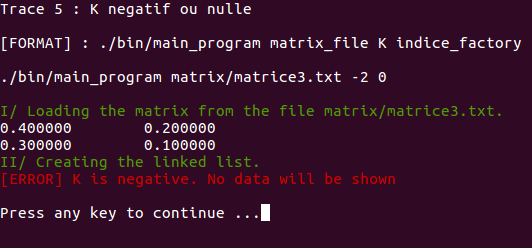
\includegraphics[scale=0.4]{trace_6.png}

figure : Trace 6
\end{center}
\begin{center}
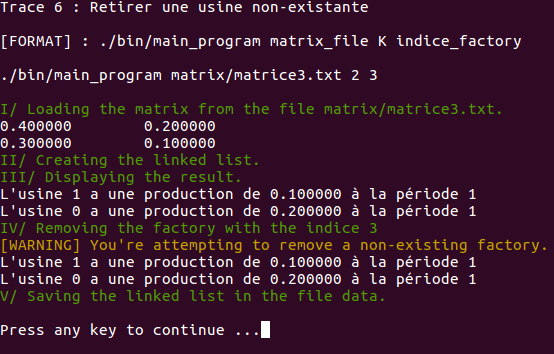
\includegraphics[scale=0.4]{trace_7.png}

figure : Trace 7
\end{center}

\begin{center}
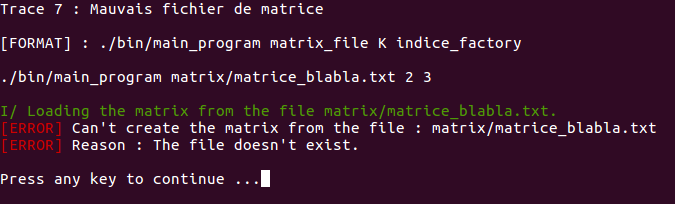
\includegraphics[scale=0.4]{trace_8.png}

figure : Trace 8
\end{center}

\begin{center}
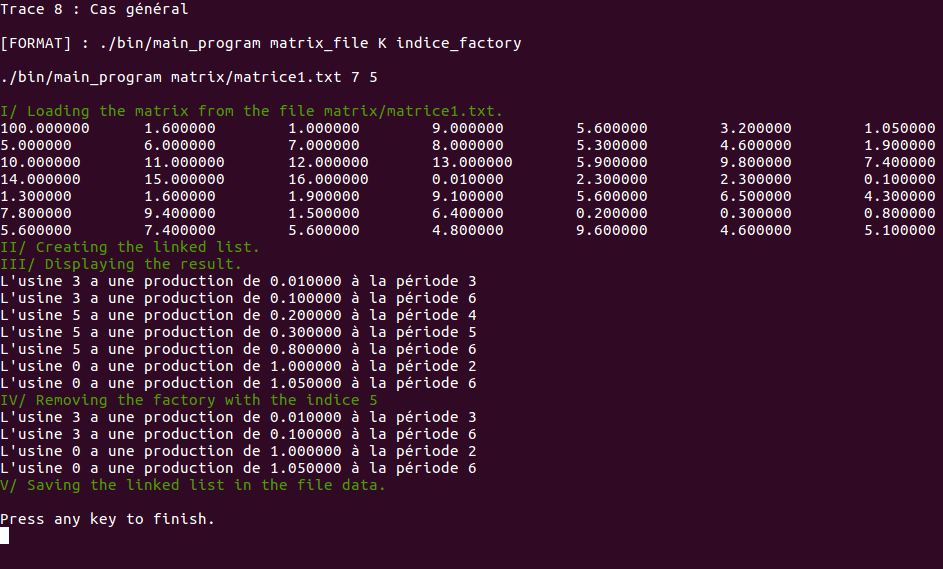
\includegraphics[scale=0.4]{trace_9.png}

figure : Trace 9
\end{center}
\end{document}